\documentclass[11pt]{article}
% -----------------------------------------------------------------------------
% Response to the reviewers of MS CPENG-8674 (major revision, October 2026).
% Draft: answers are written only for the comments addressed so far.
% Code: MODULES/review29oct_fixed | Data: Data/06Nov_FINAL_SlabS10_7D_5sensors_5modes | Figures: ./figures_final
% Orange text = notes for the authors and placeholders (remove or fill before submission).
% -----------------------------------------------------------------------------
\usepackage[a4paper,margin=2.5cm]{geometry}
\usepackage{amsmath,amssymb,bm}
\usepackage{graphicx}
\usepackage{booktabs,multirow,array,longtable,tabularx}
\usepackage{xcolor}
\usepackage{caption,subcaption}
\usepackage{float}
\usepackage{enumitem}
\usepackage{titlesec}
\usepackage{tikz}
\usetikzlibrary{decorations.pathmorphing,arrows.meta,calc,positioning,patterns,decorations.pathreplacing}
\usepackage[colorlinks=true,linkcolor=blue!50!black,citecolor=blue!50!black,urlcolor=magenta]{hyperref}

\definecolor{resp}{RGB}{25,70,170}
\definecolor{note}{RGB}{205,95,0}
\linespread{1.15}
\setlength{\parindent}{0pt}
\setlength{\parskip}{4pt}
\captionsetup{font=small,labelfont=bf,labelsep=colon}
\renewcommand{\thetable}{R\arabic{table}}
\renewcommand{\thefigure}{R\arabic{figure}}
\renewcommand{\theequation}{R\arabic{equation}}
\titleformat{\section}{\normalfont\large\bfseries}{}{0pt}{}
\titleformat{\subsection}{\normalfont\bfseries}{}{0pt}{}
\setlist{itemsep=1pt,topsep=2pt}

% --- Comment / response / action blocks (as in our previous response letters) ---
\newenvironment{rcomment}[1]{\par\bigskip\noindent\textbf{Comment\ifx&#1&\else\ #1\fi:}\ \itshape}{\par}
\newenvironment{response}{\par\smallskip\noindent\color{resp}\textbf{Response:}\ }{\par}
\newenvironment{action}{\par\smallskip\noindent\color{resp}\textbf{Action:}\ }{\par}
\newcommand{\pending}{\par\smallskip\noindent\textcolor{gray}{\textbf{Response:} \textit{pending --- this comment
has not been addressed yet.}}\par}
\newcommand{\authornote}[1]{\textcolor{note}{\textsf{[Authors: #1]}}}
\newcommand{\tbd}[1]{\textcolor{note}{\textsf{[#1]}}}
\newcommand{\lines}[1]{\tbd{lines #1}}

\newcommand{\m}{\mathbf{m}}
\newcommand{\z}{\mathbf{z}}
\newcommand{\f}{\mathbf{f}}

\begin{document}

\begin{center}
{\Large\bfseries Response to reviewer comments}\\[8pt]
\textbf{MANUSCRIPT ID:} CPENG-8674\\
\textbf{Date:} \today\\
\textbf{Title:} Uncertainty-aware damage identification in short-span bridges via physics-informed variational
autoencoder\\
\textbf{Journal:} Journal of Computing in Civil Engineering
\end{center}

\noindent\fcolorbox{note}{note!6}{\parbox{\dimexpr\linewidth-2\fboxsep-2\fboxrule}{\small\color{note}\textsf{%
\textbf{Draft status (\today).} Answers are given only for the comments addressed so far; the other comments are
reproduced with the mark ``pending''. Orange text is for the authors: notes, and placeholders for the results of the
training on the final dataset and for the line numbers of the revised manuscript. All numbers in blue come from the
final dataset (\texttt{Data/06Nov\_FINAL\_SlabS10\_7D\_5sensors\_5modes}: bridge S10 of Moliner et al., 2017, as a beam on vertical elastic supports; five sensors, five modes) and the scripts in \texttt{MODULES/review29oct\_fixed} and
\texttt{MODULES/baseline\_GaussCopula\_GaussMarginals}.}}}

\bigskip
We would like to thank the three reviewers for the time and effort they devoted to conduct this insightful review.
In the following, we answer each comment point by point. Table~\ref{tab:summary} summarizes the responses and indicates where
the corresponding changes appear in the revised manuscript. Reviewer comments are reproduced in italics, and our responses and the resulting actions are written in blue.

% =============================================================================
\section{Summary of the responses}
% =============================================================================
{\small
\begin{longtable}{p{1.55cm}p{6.0cm}p{3.0cm}p{3.6cm}}
\caption{Point-by-point summary of the responses.}\label{tab:summary}\\
\toprule
Comment & Topic & Status & Revised manuscript \\
\midrule
\endfirsthead
\toprule
Comment & Topic & Status & Revised manuscript \\
\midrule
\endhead
R1.1 & Test data from a finer FE mesh & Addressed (VAE results pending) & \lines{xx--yy} \\
R1.2 & Model uncertainty and environmental variability & Addressed & \lines{xx--yy} \\
R1.3 & Coverage values (77.2\% vs.\ 0.789) and calibration & Addressed (results pending) & \lines{xx--yy} \\
R1.4 & Comparison with Refs.\ 39 and 41 & Addressed (results pending) & \lines{xx--yy} \\
R1.5 & Out-of-distribution test cases & Addressed (results pending) & \lines{xx--yy} \\
R1.6 & Localized, mild and healthy cases; false positives & Addressed (results pending) & \lines{xx--yy} \\
R1.7 & Finer discretization and scalability & Partly addressed & \lines{xx--yy} \\
R1.8 & Reference list & Pending (issues identified) & \\
R2.1 & Utility for real bridges in the introduction & Pending & \\
R2.2 & Realistic structure and elastic bearings & Addressed & \lines{xx--yy} \\
R2.3 & Damage parametrization, support conditions and detectable bearing damage & Addressed (VAE results pending) & \lines{xx--yy} \\
R2.4 & More realistic case study; laboratory beam & Partly addressed (no laboratory data) & \lines{xx--yy} \\
R3.1 & Robustness to modelling error (mass perturbation) & Addressed (results pending) & \lines{xx--yy} \\
R3.2 & Selection of $\gamma$ on the test set & Addressed (sensitivity study pending) & \lines{xx--yy} \\
R3.3 & Prior vs.\ sampling density of the training data & Addressed & \lines{xx--yy} \\
R3.4 & Number of modes and identifiability & Addressed (VAE results pending) & \lines{xx--yy} \\
R3.5 & Flowchart of the data generation and of the offline/online phases & Addressed & \lines{xx--yy} \\
R3.6 & Notation $\mathbf{K}_{\mathrm{G}}$ in Eq.~(11) & Pending & \\
R3.7 & Number of samples $H$ & Addressed & \lines{xx--yy} \\
R3.8 & Hardware and wall-clock time & Pending & \\
\bottomrule
\end{longtable}
}

% =============================================================================
\section{Reviewer \#1}
% =============================================================================

\begin{rcomment}{}
This paper presents a physics-informed Gaussian copula variational autoencoder for uncertainty-aware damage
identification using noisy natural frequencies and mode shapes. Replacing the learned decoder with a differentiable
eigensolver appears to be an interesting approach for end-to-end training, and the manuscript is clearly written. The work
builds on the authors' earlier Gaussian copula VAE (Reference 41) and extends it by embedding the eigensolver and
increasing the latent dimensionality from 2 to 5. The current validation is based on a single five-element synthetic
beam with measurement noise, and I believe that some additional evidence would further strengthen the conclusions
regarding uncertainty quantification, reliability, and scalability. Some clarifications are needed to better understand
the method and its applications.
\end{rcomment}
%
%\begin{response}
%	
%	
%	
%The revised study is no longer based on a single five-element beam with measurement noise: the structure is a published short-span bridge on
%vertical elastic supports, the latent space has seven variables, the data include modelling
%errors, and the trained model is tested on data from two FE models. The responses below describe these changes.
%\end{response}

% -----------------------------------------------------------------------------
\begin{rcomment}{1}
The training and test data are generated using the same five-element model. Could the authors consider testing the trained model on observations generated from a finer mesh while retaining the same five damage zones and sensor locations as in the current paper? This would help assess robustness to model-form uncertainty, since field observations
may not necessarily be well represented by such a coarse discretization.
\end{rcomment}

\begin{response}
We have created a new, more realistic case study, accounting also for the other reviewer's concern. 
We designed a FE model discretized with 10 elements, which incorporates vertical support springs at both ends of the structure to represent the bearings.  
For the testing phase, we have discretized the same model into a finer mesh with 50 elements.

The latent variables correspond now to one stiffness factor per damage zone along the bridge deck (as in the original submission), plus one additional stiffness parameter per bearing (see Comment$\#2$ of Reviewer$\#2$):
\begin{equation}
\hat{\mathbf{K}}_{\mathrm{G}}(\z)=\sum_{k=1}^{5} z_k\sum_{e\in\mathcal{Z}_k}\mathbf{K}_{e}
+z_{b,L}\,\mathbf{K}_{b,L}+z_{b,R}\,\mathbf{K}_{b,R},
\label{eq:Kz}
\end{equation}
where $\mathcal{Z}_k$ is the number of elements of zone $k$ and $\mathbf{K}_{b,L}$, $\mathbf{K}_{b,R}$ contain the nominal left (L) and right (R) bearing springs.
%
%\textit{Two test sets with the same damage conditions.} The test set contains 1\,200 as-built structures (damage
%condition and as-built mass, see R1.2), observed twice with the same measurement-noise realizations. Test set A is
%computed with the 10-element model (the discretization of the decoder). Test set B is computed with a 50-element model
%(ten elements per zone), with the same five damage zones and the same five sensors. Because a finer mesh alone changes
%the modal data very little (Table~\ref{tab:budget}), test set B also represents the damage more realistically: in every
%damaged zone, the loss of stiffness is concentrated in a sub-region of random length (0.2--2.0~m, median 1.2~m) and
%position, with the same equivalent (harmonic-mean) stiffness $z_k$ of the zone (R2.3). The decoder can represent
%neither the finer mesh nor the localization, so test set B measures the robustness to model-form error. The sensors are
%placed at the zone centres instead of the zone boundaries (see R3.4). Test set A is the control. Its setting is that of
%numerical studies in which the test data come from the FE model embedded in the network; in the two-span beam of Luo et al.\
%(2025), for instance, the test samples differ from the training samples in the load, with the same FE model and parameters.
%Test set B goes beyond this control.
%
%\textit{Dataset generation.} All the datasets of the revised study are new. Table~\ref{tab:datasets} summarizes them, and Fig.~\ref{fig:flowchart} (R3.5) gives the flowchart. Every sample is
%generated in four steps:
%\begin{enumerate}[leftmargin=*,label=(\arabic*)]
%\item \emph{Damage state.} The design of experiments (R1.6) gives $\z^*\in[0.45,1]^7$: healthy structures, one to five damaged
%parameters with every location and combination equally represented, and a category drawn uniformly from the prior. The
%severities are stratified over $[0.45,0.95)$ by Latin hypercube sampling.
%\item \emph{As-built structure.} The mass of each 1~m segment is multiplied by $1+\mu_s$, $\mu_s\sim\mathcal{N}(0,0.05^2)$, with
%a new draw per sample. The decoder only knows the nominal mass (R1.2, R3.1).
%\item \emph{Modal analysis.} The eigenproblem of the as-built structure is solved with the FE model of that dataset, and the first
%five modes are kept. The training, validation and test A data use the 10-element model of the decoder. Test B uses a 50-element
%model in which the loss of stiffness of every damaged zone is concentrated in a sub-region of 0.2--2.0~m at a random position,
%with the same equivalent stiffness $z_k$ of the zone (R1.1, R2.3).
%\item \emph{Measurement noise.} We add 2.5\% to the frequencies and 5\% of the peak amplitude to each mode-shape component at the five
%sensors, as in the submitted version.
%\end{enumerate}
%Test sets A and B contain the same 1\,200 damage states, as-built structures and noise draws, so any difference between them comes
%from the FE model and the localization alone. Test set A is therefore a control, and test set B is deliberately \emph{slightly different}
%from the training data: its generator is not available to the decoder nor to the likelihood. The likelihood is calibrated once,
%on 6\,000 further structures from the training generator (R1.2), and is not recalibrated for test set B. Six further test sets
%outside the training distribution are described in R1.5.
%
%\textit{Results so far.}
%\begin{itemize}[leftmargin=*]
%\item The finer mesh alone shifts the frequencies by at most $-0.13\%$ (mode 5) and leaves the mode shapes at the sensors
%unchanged ($1-\mathrm{MAC}<10^{-5}$). The localized damage changes the frequencies by 0.8--1.5\% (standard deviation over
%the test damage states) and the mode shapes by up to $2.6\times10^{-3}$ in $1-\mathrm{MAC}$: an error of the same order
%as that of the mass deviations (Table~\ref{tab:budget}).
%\item The likelihood is calibrated on test set A: at the true damage condition, the frequency term equals 1.02 times its
%theoretical value and the mode-shape terms 0.98--1.01 times. On test set B these ratios are 1.15 and 1.00--1.36,
%because the likelihood does not include the localization (Fig.~\ref{fig:calib}): test set B is a genuine case of model
%misspecification.
%\item The exact posteriors (sequential Monte Carlo, see R1.3) of the 11 benchmark scenarios contain the true damage
%condition in their 95\% credible intervals for 68 (test set A) and 64 (test set B) of the 77 parameters. For seven
%benchmarks (P0--P4, P9 and P10), the posteriors from both test sets are almost identical (means within 0.032); for
%P5--P8, the localization changes the posterior means by 0.07--0.11. The largest change occurs in P5, where the damage of zone 1
%is combined with that of the left bearing: the standard deviation of $z_1$ falls from 0.084 to 0.028, since the localized damage
%changes how the data distribute the loss of stiffness between the end zone and the bearing (Fig.~\ref{fig:testfine}).
%\item VAE metrics on both test sets: \tbd{Table with MSE, MAE, ALL, MACE and coverage on test sets A and B}.
%\end{itemize}
%\end{response}
%
%\begin{table}[H]
%\centering\small
%\caption{Datasets of the revised study.}
%\label{tab:datasets}
%\footnotesize
%\begin{tabular}{p{2.7cm}cp{3.5cm}p{3.1cm}p{3.5cm}}
%\toprule
%Dataset & Samples & Damage states & FE model of the data & Role \\
%\midrule
%Training & 14\,000 & design of experiments & 10 elements, as-built & loss of the VAE (true damage states not used) \\
%Validation & 2\,400 & same proportions & 10 elements, as-built & model selection \\
%Test set A & 1\,200 & same proportions; 11 benchmarks & 10 elements, as-built & control \\
%Test set B & 1\,200 & the same as test set A & 50 elements, as-built, localized damage & model-form error (R1.1) \\
%Sets of R1.5 & see R1.5 & shifted, one factor per set & as test set B & outside the training distribution \\
%\bottomrule
%\end{tabular}
%\end{table}
%
%\begin{table}[H]
%\centering\small
%\caption{Relative error (\%) of the natural frequencies of the healthy bridge with respect to the 50-element model of
%the second test set.}
%\label{tab:mesh}
%\begin{tabular}{lccccc}
%\toprule
%Model & $f_1$ & $f_2$ & $f_3$ & $f_4$ & $f_5$ \\
%\midrule
%5 elements (discretization of the submitted version) & 0.010 & 0.133 & 0.474 & 0.908 & 1.323 \\
%10 elements (decoder) & 0.001 & 0.008 & 0.030 & 0.063 & 0.121 \\
%\midrule
%Frequencies of the 50-element model [Hz] & 10.649 & 38.511 & 72.958 & 108.061 & 154.507 \\
%\bottomrule
%\end{tabular}
%\end{table}
%
%\begin{figure}[H]
%\centering
%\begin{subfigure}{0.49\textwidth}\includegraphics[width=\textwidth]{figures_final/Fig_reference_posterior_P5_test.png}
%\caption{Test set A: 10-element model, uniform damage of zone 1}\end{subfigure}
%\begin{subfigure}{0.49\textwidth}\includegraphics[width=\textwidth]{figures_final/Fig_reference_posterior_P5_test_fine.png}
%\caption{Test set B: 50-element model, localized damage of zone 1}\end{subfigure}
%\caption{Exact posterior of benchmark P5 (zone 1 and left bearing damaged, $z_1=0.60$, $z_{b,L}=0.58$) computed from the
%observations of the two test sets (same damage condition, as-built mass and noise realization). The red stars mark
%the true damage condition.}
%\label{fig:testfine}
%\end{figure}
%
%\begin{action}
%The decoder now embeds a 10-element model \lines{xx--yy}; a second test set generated with a 50-element model and
%localized damage is described in \lines{xx--yy}, and Table~\tbd{x} reports the metrics on both test sets.
%\end{action}

% -----------------------------------------------------------------------------
\end{response}

\begin{rcomment}{2}
The introduction identifies model uncertainty, measurement error, and environmental variability as sources of
ill-posedness, whereas the numerical study focuses primarily on measurement noise. It would be useful to investigate how
the proposed framework handles the other sources of uncertainty or, alternatively, to discuss this point more explicitly
as a limitation of the present study.
\end{rcomment}

\begin{response}
	1. We account for the following sources of uncertainty: 
	
	A) Measrement error/noise --> already in the original submission 
	B) Modeling error: we add mass perturbation that follows a Gaussian distribution (include the equation). This is done by generating the data with nominal values and feeding the SciML model with perturbed results.  We also include the thiner mesh discretization for the test dataset to explore robustness against this modeling error
	C) we also explore an additional source of uncertainty related to limitation (sparsity) of the instrumentation system, in this case by using a reduced number of mode shapes (also requested by reviewer3). 
	D) We cannot introduce a relaistic environmental and operational variavbility in our dataset, so we acknowledge this limitation of our validation and propose experimental validation as future work to incorporate this uncertainty source. 
	
Note that the objective of our present work is not to disentangle these sources of variability (quantify each origin of uncertainty, which could be future work), but we include these sources of uncertainty to offer a realistic case sutdy and reliable validation. 
%
%	
%We agree. The revised study includes, in every dataset (training, validation and both test sets), the two sources of
%uncertainty that can be represented realistically in a synthetic setting: measurement error and modelling error.
%
%\textit{Measurement error.} As in the submitted version, we add 2.5\% noise to the identified frequencies and noise with
%a standard deviation of 5\% of the peak amplitude to each mode-shape component.
%
%\textit{Modelling error.} Each measurement comes from an as-built structure that differs from the nominal FE model
%embedded in the decoder:
%\begin{itemize}[leftmargin=*]
%\item \emph{Mass}: the mass of each 1 m segment is multiplied by $1+\mu_s$, with $\mu_s\sim\mathcal{N}(0,0.05^2)$. The uncertainty
%of the permanent loads is also considered in dynamic studies of short-span bridges (e.g., $\pm30\%$ of the ballast thickness in
%Moliner et al., 2017, about $\pm8\%$ of the mass of S10).
%\item \emph{Discretization and damage morphology} (second test set only): 50-element model in which the damage of each
%damaged zone is concentrated in a sub-region of the zone (R1.1, R2.3).
%\end{itemize}
%The mass matrix of an as-built element is therefore
%\begin{equation}
%\mathbf{M}_e^{\mathrm{ab}}=(1+\mu_{s(e)})\,\mathbf{M}_e,
%\label{eq:asbuilt}
%\end{equation}
%where $s(e)$ is the segment of element $e$. Since the deviations are defined on a grid that does not depend on the mesh,
%both test sets describe the same physical structures. The decoder keeps the nominal model: the realizations of these
%deviations are never available to the VAE.
%
%\textit{How the inference handles them.} We write the observations as
%\begin{equation}
%\m=\mathbf{g}(\z)+\bm{\delta}_{\mathrm{model}}+\bm{\epsilon}_{\mathrm{meas}},
%\label{eq:discrepancy}
%\end{equation}
%where $\mathbf{g}(\z)$ are the modal properties of the nominal model. If the likelihood ignored
%$\bm{\delta}_{\mathrm{model}}$, the stiffness factors would have to absorb the modelling error, which biases the
%estimates and makes the posterior overconfident. Instead, we estimate the statistics of
%$\bm{\delta}_{\mathrm{model}}+\bm{\epsilon}_{\mathrm{meas}}$ by simulating 6\,000 as-built structures with new random
%deviations, and include them in the likelihood: a full covariance matrix of the log-frequency errors (standard
%deviations 2.66--2.72\%, of which 0.9--1.1\% is due to the modelling error; correlations between modes below 0.14) and
%a standard deviation per mode for the mode-shape errors (0.028--0.044). This is the standard treatment of model
%discrepancy in Bayesian FE model updating, and it leaves the architecture unchanged. We verified the calibration on
%independent data generated like the training data (test set A): at the true damage condition, every likelihood term
%equals 0.98--1.02 times its theoretical value. On test set B, whose localized damage is not included in the likelihood,
%the ratios are 1.00--1.36 (Fig.~\ref{fig:calib}). Table~\ref{tab:budget} and Fig.~\ref{fig:budget} quantify each
%source: the mass deviations are the modelling error of the training data (about 1\% on the frequencies and up to
%$3.5\times10^{-3}$ in $1-\mathrm{MAC}$ for mode~5); in test set B, the localized damage adds an error of similar size
%(0.8--1.5\% on the frequencies), while the finer mesh alone only introduces a small systematic shift (at most 0.13\%).
%
%\textit{Environmental variability.} We do not simulate environmental effects. Their influence on the modal properties
%depends strongly on the structure (for instance, the stiffening of the pavement and of the bearings below freezing), and
%a realistic description requires long-term monitoring data with measured temperatures. We now discuss this explicitly
%as a limitation. The framework can incorporate such effects either as an additional, correlated term of
%$\bm{\delta}_{\mathrm{model}}$ in Eq.~\eqref{eq:discrepancy}, or by feeding the measured temperature to the encoder; we
%indicate this as future work with field data.
\end{response}

%\begin{table}[H]
%\centering\small
%\caption{Size of each source of discrepancy between the measurements and the nominal decoder (modes 1 to 5), over the
%damage states of the design of experiments: mean and standard deviation of $\log f_{\mathrm{data}}-\log
%f_{\mathrm{decoder}}$ and mean $1-\mathrm{MAC}$ of the vertical mode shapes (range over the five modes).}
%\label{tab:budget}
%\begin{tabular}{lccc}
%\toprule
%Source & Mean $\Delta\log f$ (\%) & Std $\Delta\log f$ (\%) & Mean $1-\mathrm{MAC}$ \\
%\midrule
%Finer mesh (50 elements) & $-0.001$ to $-0.125$ & $\le0.010$ & $<10^{-5}$ \\
%Mass (5\% per 1 m segment) & 0.003 to 0.049 & 0.91--1.08 & up to $3.5\times10^{-3}$ \\
%Localized damage (test set B) & $-0.07$ to 0.07 & 0.76--1.55 & up to $2.6\times10^{-3}$ \\
%\midrule
%All modelling errors, test B & $-0.040$ to 0.096 & 1.20--1.79 & up to $5.9\times10^{-3}$ \\
%Measurement noise & $\approx0$ & 2.45--2.53 & 3.0--4.3$\times10^{-3}$ \\
%\bottomrule
%\end{tabular}
%\end{table}
%
%\begin{figure}[H]
%\centering
%\includegraphics[width=\textwidth]{figures_final/Fig_model_error_budget.png}
%\caption{Size of each source of discrepancy between the measurements and the nominal decoder, per mode: frequencies
%(left) and vertical mode shapes (right).}
%\label{fig:budget}
%\end{figure}
%
%\begin{figure}[H]
%\centering
%\includegraphics[width=\textwidth]{figures_final/Fig_likelihood_calibration.png}
%\caption{Calibration of the likelihood. Left: average likelihood terms at the true damage condition divided by their
%theoretical value, for both test sets (1 means calibrated). Centre: standard deviations of the log-frequencies and of
%the unit-norm vertical mode shapes. Right: correlation between the log-frequency errors of different modes.}
%\label{fig:calib}
%\end{figure}
%
%\begin{action}
%New subsection on the sources of uncertainty and their treatment in the likelihood \lines{xx--yy}, with
%Eqs.~\eqref{eq:asbuilt}--\eqref{eq:discrepancy}, Table~\ref{tab:budget} and Figs.~\ref{fig:budget}--\ref{fig:calib};
%environmental variability discussed as a limitation in the conclusions \lines{xx--yy}.
%\end{action}

% -----------------------------------------------------------------------------
\begin{rcomment}{3}
The abstract reports 77.2\% coverage (line 32), whereas line 352 reports a value of 0.789 for nominal 95\% intervals.
Could the authors clarify how these two values are related? A value below 80\% for nominal 95\% intervals may indicate
some undercoverage. A brief discussion of how the uncertainty intervals are calibrated would therefore be helpful.
\end{rcomment}

\begin{response}
The abstract and the results section of the submitted version
report different values for the same quantity, and the value of the results section is 0.789.
\authornote{add the origin of 77.2\% only if it can be confirmed.} In the revised manuscript, a single coverage value is
reported, the abstract and the text use the same value, and the definition of the intervals is stated explicitly.

The reviewer is right that these values indicate undercoverage. We identified two causes:
\begin{enumerate}[leftmargin=*]
\item \emph{The width of the approximate posterior was not calibrated.} In the submitted loss, the frequency and MAC
terms had fixed weights ($\lambda=10$) that were not derived from the noise statistics, and the entropy term was
scaled by $\gamma^2$, with $\gamma=0.30$ selected to balance point accuracy and distributional quality. The minimizer of such a loss is a tempered posterior
whose width depends on these weights, so its credible intervals cannot be expected to reach their nominal coverage.
\item \emph{Equal-tailed intervals and the upper bound $z=1$.} An undamaged parameter lies close to the upper bound of
the support, where its posterior accumulates. An equal-tailed (central) 95\% interval excludes the upper 2.5\% of the
probability, and therefore often excludes a true value close to 1, even when the posterior is correct. In the revised
test set, 67\% of the parameters are undamaged ($z^*\ge0.95$) and 18\% lie above the 97.5\% quantile of the prior. As a
result, even the prior, which ignores the data, reaches only 81\% coverage with central 95\% intervals on this test set.
A coverage of central intervals below 80\% is therefore not necessarily a sign of a poorly calibrated posterior.
\end{enumerate}

We made the following changes:
\begin{itemize}[leftmargin=*]
\item \emph{Calibrated likelihood.} The data terms of the loss are the negative log-likelihood of the frequency and
mode-shape errors, with the variances calibrated by simulation and verified on independent data (R1.2):
\begin{equation}
\mathrm{NLL}(\z;\m)=\tfrac12\,\mathbf{d}^{\top}\bm{\Sigma}_f^{-1}\mathbf{d}
+\sum_{j=1}^{n_m}\frac{1-\mathrm{MAC}_j(\bm{\Phi},\hat{\bm{\Phi}}(\z))}{2\,s_{v,j}^2},\qquad
\mathbf{d}=\log\f-\mathbf{b}-\log\hat{\f}(\z).
\label{eq:nll}
\end{equation}
For unit-norm mode shapes perturbed by Gaussian noise, $1-\mathrm{MAC}_j$ equals the squared noise component
perpendicular to the shape, so the second term is the Gaussian log-likelihood of that component.
\item \emph{No tempering ($\gamma=1$).} With a uniform prior on $\mathcal{S}=[0.45,1]^7$, the loss
\begin{equation}
\mathcal{L}(\bm\theta)=\frac1N\sum_{i=1}^N\Big(\mathbb{E}_{q}\big[\mathrm{NLL}(\z;\m_i)\big]
-\gamma^2\,\mathcal{H}\big[q_{\bm\zeta_{\bm\theta}}(\z|\m_i)\big]\Big)
\label{eq:loss}
\end{equation}
is the negative ELBO for $\gamma=1$ (up to a constant), and its minimizer is the Bayesian posterior within the
variational family. $\mathcal{H}$ is the entropy of the copula model: the copula part, $\frac12\log\det\mathbf{R}$, and
the entropies of the truncated Gaussian marginals are both computed exactly.
% [ln z omitted in this revision, kept for later] the entropies of the marginals (Eq.~\eqref{eq:marginal}) are both computed exactly.
\item \emph{Exact credible intervals.} The marginals of the approximate posterior are truncated Gaussian distributions with a
closed-form CDF $F_{q,e}$, so we compute the probability integral transform $u_{t,e}=F_{q,e}(z^*_{t,e})$ of every true
value exactly. The true value lies inside the equal-tailed interval of level $p$ if $|2u_{t,e}-1|\le p$, and inside the
highest-density region of level $p$ if the posterior probability of $\{z: q_e(z)>q_e(z^*_{t,e})\}$ does not exceed $p$.
\item \emph{Reliability diagrams.} We compute the empirical coverage at 19 nominal levels, from $p=0.05$ to $p=0.95$ in
steps of 0.05, and the MACE, with both types of intervals, for all parameters and separately for deck zones and bearings, for damaged and
undamaged parameters, and for the test scenarios drawn from the prior, where a Bayesian posterior must be calibrated by
construction.
\item \emph{Reference posterior.} We compare the VAE with the exact posterior obtained by sequential Monte Carlo with
the same likelihood and prior. It starts from samples of the prior, introduces the likelihood gradually through an
exponent that grows from 0 to 1, and never uses the true damage condition. This separates the approximation error of
the VAE from the effect of the bounds described above.
\end{itemize}

\tbd{Results on the final dataset: coverage and MACE with both types of intervals (all, deck zones, bearings, damaged, undamaged,
scenarios drawn from the prior); reliability diagram; VAE vs.\ exact posterior vs.\ prior on the scenarios drawn from the prior.}
\end{response}
\authornote{decide which single value goes in the abstract, and confirm that the submitted version used central intervals.}

\begin{action}
Abstract and Section~\tbd{x} corrected so that they report the same value \lines{xx--yy}; new paragraph on the
calibration of the likelihood and the definition of the intervals \lines{xx--yy}; new reliability diagram (Fig.~\tbd{x})
and coverage table (Table~\tbd{x}).
\end{action}

% -----------------------------------------------------------------------------
\begin{rcomment}{4}
References 39 (Gaussian mixture autoencoder) and 41 (Gaussian copula VAE) introduce closely related methods that could
potentially serve as useful baselines. A comparison with these approaches would help assess the benefits of the proposed
strategy more effectively.
\end{rcomment}

\begin{response}
Some comments for this:

1. We can compare against a Gaussian copula VAE as in our previous paper: that paper trained teh decoder as a neural network (Surrogate model that is pre-trained before training the inverse). Then this architecture component is frozen and teh training is conducted to optimize the inverse approximator. So rather than using the eigenhsolver it uses a surrogate. we could compare these approaches in terms of results' accuracy and computational cost. Adding an extra NN makes the convexity of the solution space more difficult problably? and we need to estimate more parameters, and add an extra source or error, plus we need the two-step training in terms of computation.
2. we could compare against teh Gaussian mixture with same eigenvalue solver-based decoder. This would constitute a comparison of teh efficiency of the proposed latent space distribution model (apprxoximaiton of the true posterior): when using the Gaussian mixture without copula, we may miss correlations, and we will incccur in larger number of parameters to be estimated as dimensionality increases, plus more computational cost. 

If we do this, we need to create the surrogate forward NN  and train it for case 1 and obtain all the results for case 1.   
For comparison 2 we must use a sum of K = 5 gaussians without copula and see what we obtain for full-covariance matrix assumption. 



\end{response}

%
%\authornote{Without the change of variable to $\ln z$, the proposed model and the baseline of Ref.~41 have the same variational family (Gaussian copula with truncated Gaussian marginals), so this comparison must be redefined, e.g., by what distinguishes Ref.~41 (decoder and loss), or by comparing only with Ref.~39. The commented text below keeps the description of the $\ln z$ marginals.}
%% \item \emph{Same methodology, with the Gaussian marginals in $\ln z$.} The encoder, the Gaussian copula that models the
%% dependence between parameters, the differentiable eigenvalue decoder and the ELBO loss are those of the submitted
%% version, and each parameter still has one truncated Gaussian marginal. The only change in the variational family is that
%% this Gaussian now describes $y_d=\ln z_d$ instead of $z_d$, so that each marginal is a truncated log-normal distribution on
%% the support $[0.45,1]$ of the stiffness factors:
%% \begin{equation}
%% q_d(z_d|\m)=\frac{\varphi\big((\ln z_d-\mu_d)/\sigma_d\big)}{\sigma_d\,Z_d\,z_d},\qquad
%% F_d(z_d|\m)=\frac{\Phi\big((\ln z_d-\mu_d)/\sigma_d\big)-\Phi(\alpha_d)}{Z_d},
%% \label{eq:marginal}
%% \end{equation}
%% with $\alpha_d=(\ln 0.45-\mu_d)/\sigma_d$, $\beta_d=-\mu_d/\sigma_d$ and $Z_d=\Phi(\beta_d)-\Phi(\alpha_d)$, where
%% $\varphi$ and $\Phi$ are the standard normal density and CDF, and $\mu_d$ and $\sigma_d$ are outputs of the encoder. The
%% copula is not affected, because a copula does not change under monotone transformations of the variables. The prior
%% remains uniform in $\z$ and the likelihood is unchanged, so the target is the same Bayesian posterior. The samples and the
%% entropy keep closed forms: $z_d=\exp\big(\mu_d+\sigma_d\Phi^{-1}(\Phi(\alpha_d)+u_dZ_d)\big)$ for the copula variable
%% $u_d$, and $\mathcal{H}[z_d]=\mathcal{H}[y_d]+\mathbb{E}[y_d]$, with the entropy and the mean of the truncated normal
%% distribution.
%%
%% The reason for this choice is the structure of the problem. The frequency term of the likelihood is Gaussian in the
%% logarithm of the frequencies (Eq.~\eqref{eq:nll}) and, for fixed mode shapes, the squared frequencies are linear in the stiffness factors
%% (Eq.~\eqref{eq:Kz}). When one parameter dominates a mode, $\ln f_j\approx\frac12\ln z_k+\text{const.}$, so the
%% errors are approximately Gaussian in $\ln z_k$. The argument is only approximate when several parameters contribute to a
%% mode, so we checked it on the validation set, without the encoder, against the exact posteriors of 131 observations (917
%% marginals). For marginals whose bell lies inside the support, the median skewness is $+0.24$ in $z$ and $+0.02$ in
%% $\ln z$. The mean Wasserstein-1 distance of the best fit to the exact marginals is 0.0025 for one Gaussian in $z$ and
%% 0.0010 for one Gaussian in $\ln z$. The location is allowed to lie outside the support, $\mu_d\in(\ln0.45-3\sigma_d,\,
%% 3\sigma_d)$, so that the density can keep rising up to a bound, as it does for healthy parameters; truncation keeps every
%% sample in $[0.45,1]$.
%% \tbd{Validation negative ELBO of the marginals in $z$ and in $\ln z$ with identical training (R1.4).}
%\authornote{(i) code in the folders baseline\_GaussCopula\_GaussMarginals (submitted model and proposed model:
%GCTN\_model.py), baseline\_GaussMixture\_K5 and model\_comparison of MODULES. (ii) Two random seeds are needed for the proposed model. (iii) All three models must be trained with the rule of R3.2.}
%
%\begin{action}
%New subsection ``Comparison with related methods'' \lines{xx--yy}, with Table~\tbd{x} and Fig.~\tbd{x}.
%\end{action}

% -----------------------------------------------------------------------------
\begin{rcomment}{5}
All test cases appear to be sampled from the same distribution as the training data. It would be helpful to include several additional cases where the test data fall outside the training distribution to illustrate how the proposed method behaves under distribution shift.
\end{rcomment}

\begin{response}
	
Here we need to include now a detailed explanation on (a) how the training/validation samples were createed, according to whihc distribution etc., and (b) how the additional six test "sets" outside the training distribution. Right now, i do not know what are you talking about, so you must explain this. 
I do not know what they mean by ssampled from the same distribution, but we need to give a proper response to this issue. How do we make sure that some test examples do not belong to the training set? Despite sharing the interval of addmissible values (0.45,1). 

This needs clarification, and better explanations so that we know all our test cases to what they correspond and why they indeed differ from the training ones. 



We agree. Besides test set B, which already differs from the training data in its FE model and damage morphology (R1.1),
we added six test sets outside the training distribution. Each one changes a single factor with respect to test set B
and, except for the second, contains the same structures and noise realizations, so that every change in the results is
caused by the shift alone. The VAE is not retrained, and the decoder and the likelihood remain those of the training
data:
\begin{enumerate}[leftmargin=*]
\item \emph{Damage beyond the training and prior range}: the damaged deck zones have $z\in[0.30,0.45)$.
\item \emph{Damage not aligned with the zones}: one or two defects of 0.2--0.6~m with the local stiffness reduced to
25--70\% of its nominal value, at random positions, including across zone boundaries and next to the supports.
\item \emph{Noise twice the assumed level}: 5\% on the frequencies and 10\% on the mode shapes.
\item \emph{Modelling error twice the assumed level}: 10\% mass deviations.
\item \emph{Systematic modelling error}: 5\% of additional mass not included in the model (e.g., a new surfacing layer).
\item \emph{Bearings stiffer than nominal} (by a factor of 3, e.g., aged bearings), outside the support of
the prior. Bearings may stiffen with age (Erduran et al., 2022), and the updated vertical stiffness of most bearings of
an existing bridge exceeded its nominal value (El-Borgi et al., 2005).
\end{enumerate}
For each set, we report the metrics of R1.3, the detection and false-alarm rates, and the exact posteriors of 40 cases.
Comparing the VAE with the exact posterior separates two effects: the misspecification of the Bayesian model itself,
which affects any method that uses the same model and likelihood, and the amortization error of the encoder for inputs
that differ from its training data, which we measure with the Pareto-$\hat{k}$ diagnostic and the distance to the exact
posteriors.
\tbd{Results: summary table, reliability diagrams and examples.}
\end{response}
\authornote{code: MODULES/review29oct\_fixed/ood\_study.py (to be run on the final dataset).}

\begin{action}
New subsection on the behaviour under distribution shift \lines{xx--yy}, with Table~\tbd{x} and Fig.~\tbd{x}.
\end{action}

% -----------------------------------------------------------------------------
\begin{rcomment}{6}
The paper introduces damage by sampling from a uniform distribution (line 323), which appears to result in substantial
stiffness reduction in most or all five elements simultaneously. Since structural damage is often localized, it would be
valuable to also evaluate healthy cases and cases with mild damage affecting only one or two elements. Reporting the
corresponding false-positive behavior would further support the manuscript's emphasis on early damage identification.
\end{rcomment}

\begin{response}
We have generated a new dataset based on this comment, which now includes localized damage scenarios rather than uniformly distributed ones. 
The revised design of experiments (DoE) is a stratified mixture of scenario categories
(Table~\ref{tab:doe}, Fig.~\ref{fig:doe}): healthy structures, one, two, three, or four to five damaged parameters, and a category drawn uniformly over the support of the prior. 
Within each category, every damage location (five zones and two bearings) and every combination of locations appears the same number of times.
The severities of the damaged parameters are stratified (Latin hypercube) over $[0.45,0.95)$, which covers mild to severe damage without gaps, and
the undamaged parameters lie in $[0.95,1]$. 
The validation and test sets follow the same proportions.

The first eleven test samples are benchmark scenarios (Fig.~\ref{fig:doe}, bottom right): a healthy bridge (P0),
damage in a single zone with severe, moderate, mild and very mild severity (P1, P2, P3 and P10, the latter with
$z_4=0.90$), degradation of one bearing (P4), and combined scenarios (P5 to P9).

To quantify false positives, a parameter is declared damaged when the upper limit of its 95\% credible interval falls below the damage threshold 0.95. We report the false-alarm rate (fraction of undamaged parameters declared damaged) and the detection rate (fraction of parameters with $z^*<0.90$ asigned to be damaged), for the whole test set and per category, together with the posteriors of the healthy and mildly damaged benchmarks.
\tbd{False-alarm and detection rates of the final model; posteriors of P0, P3 and P10.}
\end{response}

\begin{table}[H]
\centering\small
\caption{Scenario categories of the design of experiments (14\,000 training samples).}
\label{tab:doe}
\begin{tabular}{lccl}
\toprule
Category & Share & Training samples & Damaged parameters \\
\midrule
Healthy & 10\% & 1\,400 & none \\
Single damage & 30\% & 4\,200 & one (each of the seven locations equally often) \\
Double damage & 25\% & 3\,500 & two (all 21 pairs) \\
Triple damage & 15\% & 2\,100 & three (all 35 triples) \\
Multiple damage & 10\% & 1\,400 & four or five (all 56 combinations) \\
Uniform & 10\% & 1\,400 & $\z\sim\mathcal{U}[0.45,1]^7$ (whole support of the prior) \\
\bottomrule
\end{tabular}
\end{table}

\begin{figure}[H]
\centering
\includegraphics[width=0.95\textwidth]{figures_final/Fig_DoE_balance.png}
\caption{Design of experiments: number of training samples in which each parameter is damaged, per category;
histogram of the stiffness reduction factors; number of damaged parameters per sample in the training, validation and
test sets; and the eleven benchmark scenarios.}
\label{fig:doe}
\end{figure}

\begin{action}
New description of the DoE \lines{xx--yy} with Table~\tbd{x} and Fig.~\tbd{x}; false-alarm and detection rates reported
in \lines{xx--yy}.
\end{action}

% -----------------------------------------------------------------------------
\begin{rcomment}{7}
How does the proposed approach perform when the system is discretized more finely? The conclusion (lines 399-403)
refers to scalability to large-scale infrastructure. Could the authors comment on the expected computational and
statistical scaling of the method for systems with hundreds of elements, particularly given that the number of copula
correlation parameters and the computational cost of the eigensolver may both increase with problem size?
\end{rcomment}

\begin{response}
We have created a more finely discretized FE model (50 elements) for testing purposes.
We train our model with a 10DOF FE model and then use the finer mesh FE model for the testing phase. 

the scalability problems will appear as we attempt to identify more localized damage in complex strictures, and not so much in the number of elements: we may have 50 elements, but five target damage zones, which results in a reduced number of parameters to approximate the target posterior. 
However, if we wanted to describe a 50-dimensional posterior (one daamage zone per element, reduced damage locations, localized damaged), this will considerably increase the dimensionality of the parameters to be estimated and introduce scalabilitty problems. However, the use of the copula approach intends to benefit in such situations by reducing the number of parameters to  be estimated in multivariate cases compared to other approaches such as Gaussian mixture.


So we need to comment (a) in the results section: the capability that we have to identify the damage in a finely discretized model that was NOT used in training . (this provided good results)

In the conclusions we must discuss what I mention about the scalability problems not because of the size of the FE model but for the level of localization (idneitification) of damage. 

%In the revised formulation, the FE discretization is decoupled from the damage parametrization. The latent variables
%are the stiffness factors of the damage zones and bearings, and each zone may contain any number of elements
%(Eq.~\eqref{eq:Kz}). The copula has $d(d-1)/2$ correlation parameters for $d$ latent variables (21 for $d=7$), a number
%that depends on the number of damage zones and not on the number of elements. In the revised study, the decoder uses 10
%elements (22 DOFs) instead of 5 without changing the latent dimension, and the trained model is tested on data from a
%50-element model (102 DOFs) with localized damage, see R1.1.
%
%\tbd{Results of the VAE on test set B.}
\end{response}
%\authornote{discussion of the computational and statistical scaling still to be written: (i) structured correlation
%matrices (banded, low-rank plus diagonal) keep the number of copula parameters linear in $d$; (ii) the decoder solves
%one symmetric eigenproblem of size $n_{\mathrm{dof}}$ per sample, $O(n_{\mathrm{dof}}^3)$, batched; reduced-order
%models or iterative solvers for the first $n_m$ modes would reduce this cost for hundreds of elements; (iii) report the
%measured time per epoch for different meshes (to be measured with the final training; 22-DOF decoder and 1\,536
%eigenproblems per step, solved on the CPU in double precision).}
%
%\begin{action}
%New paragraph on the decoupling of the mesh and the latent space \lines{xx--yy}. \tbd{scaling discussion.}
%\end{action}

% -----------------------------------------------------------------------------
\begin{rcomment}{8}
A few references may benefit from a final consistency check. In particular, Reference 77 appears to contain placeholder fields, and some references seem to be duplicated.
\end{rcomment}
We have revised the references list and corrected the errors. 

\pending
\authornote{issues found in the submitted manuscript: Ref.~77 (Ding et al., 2026) has placeholder fields (author
``J.~Author'', journal ``Journal Name'', vol.~XX, pp.~XX--XX); Refs.~18 and 27 are the same paper (Simoen et al., 2015);
Refs.~56 and 57 are two editions of Przemieniecki's book; Kingma and Welling (2013) and Mottershead (1993) are listed but
not cited. The references must also follow the author--date style required by ASCE.}

% =============================================================================
\section{Reviewer \#2}
% =============================================================================

\begin{rcomment}{}
The paper presents a method based on physics-informed Gaussian copula variational autoencoder (PI-GCVAE) for
structural health monitoring (SHM) of simply supported bridges. The novelty lies in embedding a differentiable numerical
eigenvalue solver directly into the VAE architecture. The method is then demonstrated on a numerical study. The current
study is on a topic of relevance and general interest to the readers of the journal. However, I think the paper needs to
address several significant concerns and in my opinion has not yet reached the maturity to be published in CPENG
journal.
\end{rcomment}
%
%\begin{response}
%The concerns about the structural model motivated the main changes of the
%revised case study: a published short-span bridge on vertical elastic supports, a
%damage parametrization that includes the supports, two FE models (the second with localized damage), and modelling
%errors in all the data. We describe them below.
%\end{response}

% -----------------------------------------------------------------------------
\begin{rcomment}{1}
Introduction. The introduction is written well, but too much effort has been put on proving the methodological novelty. I recommend focusing also on the utility to justify the value of the method for real bridges, as it seems that the generalization of the approach is very difficult to other types of bridges considering the limitations of simply
supported bridge formulation and damage parametrization approach.
\end{rcomment}
\pending
\authornote{points for the revised introduction: the case study is now a published short-span bridge on elastic supports
whose damage is identifiable (R2.2); the formulation applies to any linear FE model whose stiffness is a weighted sum of
parameter matrices, so continuous bridges (intermediate bearings or piers) or other damage zones only add parameters;
the value for owners is a calibrated probability of damage per zone and bearing, which supports inspection
decisions.}

% -----------------------------------------------------------------------------
\begin{rcomment}{2}
Methodology. The assumption of simply-supported beam for single span bridges is not realistic. 
The majority of them sits on elastic bearings whose effects are demonstrated in the literature. 
The formulation should at least include the vertical springs at the ends.
\end{rcomment}
We have designed a new, more realistic, single-span bridge model that includes elastic bearings at both ends. 
We represent the (support conditions) elastic bearings by vertical srpings with an assigned stiffness value.  
The nominal values have been chosen following similar works existing in the literature (mention the papers that we used to decide the nominal values here). 

We now consider two discretization levels: 
for training, we assume 10DOFs with 5 damaged regions (two elements per zone) along the bridge deck, and consider also the possiblity of the bearings to suffer damage, resulting in a 7-dimensional latent space. 
For testing, we consider a much finer discretization inti 50 elements (each zone along the deck now contains 10 elements). This allows us to account for model discrepancy. we also introduced a model discrepancy in teh form of a mass perturbation.

Note: this needs to be writen well and better organized, but right now it incldues the relevant information to respond the reviewers. 

The figure that you include does not show the 10-element discretization, it shows only the five zones, but withot clarifying it very well in the image. We need to make sure that the reviewers understand that in the coarsely discretized model we consider 10 elements and five zones. 

Also, you include many explanations related  to the effect of bearings, scope of the model... .many things that are very far from what the reviewer is asking and thus, unnecessary. He wants us to include the vertical bearings: we have done it! We only need to explain well how we model them and what nominal values we use a baseline (and why, literature from where we took the values). 
Besides the FE model figure, I do not want to visualize any figure in this response (related to results nor anything). This is not what the reviewr asked. Do not get crazy. 


\begin{response}
We agree. Most short and medium span bridges rest on elastomeric bearings, whose vertical flexibility lowers the natural
frequencies and modifies the mode shapes, especially those of the higher modes (Zuk, 1962; Moliner et al., 2017; Erduran et al.,
2022). The revised model replaces the simple supports by a vertical spring at each end. No degree of freedom is removed, so the
model has $2(n_{\mathrm{el}}+1)$ DOFs, and the ends rotate freely, as in Erduran et al.\ (2022). Each spring has its own stiffness
factor (Eq.~\eqref{eq:Kz}), so damage can occur in the deck and at the supports.

\textit{Choice of the bridge.} We did not want to define a new structure, so we adopted a published one. Moliner et al.\ (2017)
derive a set of representative short-span bridges from existing structures, and they describe the bearings by
$\kappa=EI\pi^3/(K_vL^3)$, with $\kappa=0$, 0.05 and 0.1. We use their slab bridge S10 with $\kappa=0.05$ and the nominal values of
modulus and mass (Table~\ref{tab:specs}). This also corrects a second limitation of the submitted version: with its academic
section, any realistic bearing would have been effectively rigid (Table~\ref{tab:old_new}). The resulting case study is shown in Fig.~\ref{fig:bridge} and Table~\ref{tab:specs}.

\begin{figure}[H]
\centering
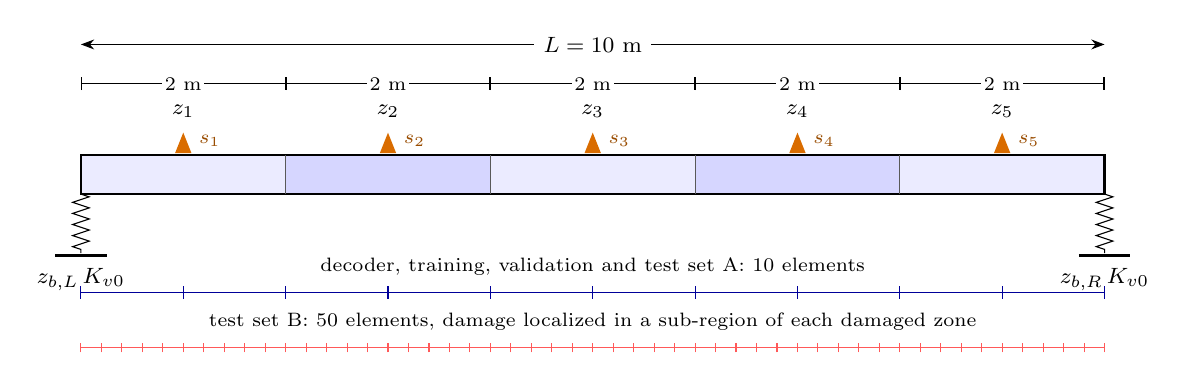
\begin{tikzpicture}[>=Stealth,font=\small,x=1.3cm]
  \foreach \i/\c in {0/blue!8,1/blue!16,2/blue!8,3/blue!16,4/blue!8}{
    \fill[\c] (2*\i,0) rectangle (2*\i+2,0.5);
    \node[font=\footnotesize] at (2*\i+1,1.05) {$z_{\the\numexpr\i+1\relax}$};
    \draw[|-|] (2*\i,1.4) -- (2*\i+2,1.4) node[midway,fill=white,font=\scriptsize,inner sep=1pt] {2 m};
  }
  \draw[thick] (0,0) rectangle (10,0.5);
  \foreach \x in {2,4,6,8} \draw[gray!70!black] (\x,0) -- (\x,0.5);
  \draw[<->] (0,1.9) -- (10,1.9) node[midway,fill=white,font=\footnotesize] {$L=10$ m};
  \foreach \x/\k in {1/1,3/2,5/3,7/4,9/5}{
    \fill[orange!85!black] (\x-0.08,0.52) -- (\x+0.08,0.52) -- (\x,0.78) -- cycle;
    \node[font=\scriptsize,orange!60!black,anchor=west] at (\x+0.06,0.68) {$s_{\k}$};
  }
  \foreach \x/\lab in {0/{L},10/{R}}{
    \draw[decorate,decoration={zigzag,segment length=4,amplitude=3}] (\x,0) -- (\x,-0.75);
    \draw[thick] (\x-0.25,-0.78) -- (\x+0.25,-0.78);
    \node[font=\footnotesize,anchor=north] at (\x,-0.82) {$z_{b,\lab}\,K_{v0}$};
  }
  \node[font=\scriptsize,anchor=south] at (5,-1.15) {decoder, training, validation and test set A: 10 elements};
  \draw[blue!60!black] (0,-1.25) -- (10,-1.25); \foreach \k in {0,...,10} \draw[blue!60!black] (\k,-1.33) -- (\k,-1.17);
  \node[font=\scriptsize,anchor=south] at (5,-1.85) {test set B: 50 elements, damage localized in a sub-region of each damaged zone};
  \draw[red!65] (0,-1.95) -- (10,-1.95); \foreach \k in {0,...,50} \draw[red!65] (\k*0.2,-2.01) -- (\k*0.2,-1.89);
\end{tikzpicture}
\caption{Revised case study: bridge S10 of Moliner et al.\ (2017) as a beam on vertical elastic supports. The seven unknowns are the
stiffness factors of the five 2~m deck zones and of the two supports, all in $[0.45,1]$. Five accelerometers $s_1,\dots,s_5$ lie at
the zone centres.}
\label{fig:bridge}
\end{figure}

\begin{table}[H]
\centering\small
\caption{Main specifications of the revised case study and origin of each value.}
\label{tab:specs}
\footnotesize
\begin{tabular}{p{3.5cm}p{6.8cm}p{4.5cm}}
\toprule
Item & Value & Origin \\
\midrule
Bridge & reinforced concrete slab deck S10, $L=10$~m, $B=11.6$~m, $h=0.77$~m & Moliner et al.\ (2017), Table 2 \\
Elastic modulus & $E=3.4849\times10^{10}$~Pa (nominal) & Moliner et al.\ (2017), Table 3 \\
Mass & 31\,301~kg/m (nominal, with ballast, sleepers and rails) & Moliner et al.\ (2017), Table 2 \\
Bending stiffness & $EI=1.54\times10^{10}$~N\,m$^2$, with $I=Bh^3/12$ & from the values above \\
Supports & vertical springs, $\kappa=EI\pi^3/(K_{v0}L^3)=0.05$, so $K_{v0}=9.5\times10^{6}$~kN/m per support; free end rotations &
$\kappa$: Moliner et al.\ (2017); range and free rotations: Erduran et al.\ (2022) \\
Unknowns & $\z\in[0.45,1]^7$: five deck zones and two supports & our choice; same range in Luo et al.\ (2025) \\
Decoder & Euler--Bernoulli beam, 10 elements, 22 DOFs, nominal mass & our choice, Table~\ref{tab:mesh} \\
Observations & first five frequencies (10.65, 38.5, 73.0, 108.1 and 154.5~Hz for the healthy bridge) and vertical mode shapes at five sensors & our choice, R3.4 \\
Noise & 2.5\% on the frequencies; 5\% of the peak amplitude on the mode shapes & submitted version \\
Modelling error & mass of each 1~m segment $\mathcal{N}(0,0.05^2)$; test set B: finer mesh and localized damage & assumption, cf.\ $\pm30\%$ of the ballast thickness in Moliner et al.\ (2017) \\
\bottomrule
\end{tabular}
\end{table}


\begin{table}[H]
\centering\small
\caption{Structure of the submitted version and revised case study. Energy and frequency changes for modes 1--5; frequency change
for a 55\% loss of stiffness of one support.}
\label{tab:old_new}
\footnotesize
\begin{tabular}{p{5.6cm}p{3.9cm}p{5.1cm}}
\toprule
 & Submitted version & Revised case study (S10) \\
\midrule
Bending stiffness $EI$ & $1.75\times10^{6}$~N\,m$^2$ & $1.54\times10^{10}$~N\,m$^2$ \\
Mass per unit length & 39~kg/m & 31\,301~kg/m \\
Supports & rigid, simple supports & vertical springs, $\kappa=0.05$ \\
First frequency (EN~1991-2 range: 8.0--16.9~Hz) & 3.3~Hz (outside) & 10.65~Hz (inside) \\
Mid-span deflection under permanent load & 28.7~mm ($L/350$) & 2.8~mm ($L/3\,600$) \\
Energy in the vertical springs & -- & 6.1--56.3\% \\
Frequency change, $z_{b,L}=0.45$ & -- & $-1.9$ to $-12.3$\% \\
\bottomrule
\end{tabular}
\end{table}

\textit{Effect of the bearings.} The sensitivity of the squared frequency of a mode to the stiffness of a spring equals
the fraction of the modal strain energy stored in that spring. The springs store 6--56\% of the strain energy of the five modes
(Table~\ref{tab:bearing_energy}), and they lower the first frequency from 10.98~Hz (simple supports) to 10.65~Hz ($-3\%$).
With the same model and $\kappa=0.1$, the reduction is 5.9\%, which agrees with the maximum of 6\% reported by Moliner et al.\ (2017)
for their slab bridges; our 10.65~Hz also lies within the band of EN~1991-2, like all their bridges, and the higher modes are the
most affected, as they report. Consequently, a 55\% loss of stiffness of one bearing changes the frequencies by 1.9--12.3\% and the
mode shapes by up to 0.11 in $1-\mathrm{MAC}$, well above the identification noise (2.5\% and about $4\times10^{-3}$) from mode 2
onwards. For instance, the exact posterior of benchmark P4 (left bearing, $z_{b,L}=0.55$) has mean 0.52 and standard deviation
0.03, against 0.16 for the prior (Fig.~\ref{fig:bearing}).

\textit{Supporting literature.} Table~\ref{tab:lit} gives the support of each decision. Physics-encoded identification has also been
applied to a two-span numerical beam whose unknowns include support springs (Luo et al., 2025). That beam fixes the vertical
displacement of the ends, with rotational springs there and a vertical spring only at the middle support, and it verifies a
time-domain method. We share its formulation of the stiffness matrix, but we place vertical springs at the ends, as this comment
requests; its vertical spring at an intermediate support shows that a continuous bridge would only add parameters to Eq.~\eqref{eq:Kz}.

\textit{Scope of the model.} The planar beam represents the longitudinal bending modes. Moliner et al.\ (2017) use an orthotropic plate for
their numerical results, since the deck is wider than its span. In S10, the first torsion mode lies at 1.53 times the first bending mode, against
1.08--1.12 in their girder bridges, so it is well separated, but torsional and transverse modes are outside the scope of the present
model and would have to be excluded when pairing measured modes. Shear deformation is neglected, as in the beam models above, while the mass
matrix includes rotary inertia. Mode 5 has half-waves of 2~m in a 0.77~m deep deck, so the highest frequencies would be lower with shear;
since the same beam theory produces the data and the decoder, this does not affect the conclusions of the numerical study, and with field data
it would be part of the model discrepancy of R1.2. Three modes are also studied (R3.4).

\begin{table}[H]
\centering\small
\caption{Modelling decisions of the revised case study and their support in the literature.}
\label{tab:lit}
\footnotesize
\begin{tabular}{>{\raggedright\arraybackslash}p{3.1cm}>{\raggedright\arraybackslash}p{4.3cm}%
>{\raggedright\arraybackslash}p{7.4cm}}
\toprule
Decision & Revised case study & Literature \\
\midrule
Bridge & S10: $L=10$~m, $h=0.77$~m, 31\,301~kg/m & taken from Moliner et al.\ (2017), derived from existing structures \\
Deck model & Euler--Bernoulli beam, vertical bending modes & beam on elastic supports (Zuk, 1962; Moliner et al., 2017; Erduran et al., 2022) \\
Bearings & linear vertical springs at both ends & equivalent vertical stiffness (Moliner et al., 2017); vertical springs (Erduran et al., 2022); linear springs updated
from modal data (El-Borgi et al., 2005) \\
End rotations & free & free end rotations (Erduran et al., 2022) \\
Vertical stiffness & $\kappa=0.05$, $K_{v0}=9.5\times10^{6}$~kN/m & $\kappa=0$, 0.05, 0.1 (Moliner et al., 2017); commercial bearings
$10^{5}$--$10^{7}$~kN/m (Erduran et al., 2022) \\
Effect of the bearings & $-3\%$ on $f_1$ ($-5.9\%$ for $\kappa=0.1$), higher modes most affected & up to 6\% for $\kappa=0.1$ in slab bridges, higher modes most affected (Moliner et
al., 2017; Erduran et al., 2022); larger in shorter spans (Zuk, 1962) \\
Damage parameters & stiffness factors of the deck zones and the supports & elastic modulus of the deck and bearing stiffness as updating parameters
(El-Borgi et al., 2005); modulus reduced by 10--20\% for cracking (Moliner et al., 2017); bearing deterioration detected from frequencies
and MAC (Fayyadh and Abdul Razak, 2012) \\
Stiffness matrix & linear in the unknown factors (Eq.~\eqref{eq:Kz}) inside a differentiable decoder & $\mathbf{K}=\sum_i\theta_i\mathbf{K}_i$ inside a differentiable network, with span and
support-spring factors (Luo et al., 2025) \\
Range of the factors & $[0.45,1]$ & $[0.45,1]$ in the laboratory damage identification of Luo et al.\ (2025) \\
Uncertain mass & 5\% per 1~m segment (our assumption) & $\pm30\%$ of the ballast thickness (Moliner et al., 2017) \\
\bottomrule
\end{tabular}
\end{table}
\authornote{confirm that the beam of the submitted version had $I=8.33\times10^{-6}$~m$^4$ and $A=0.005$~m$^2$. Check in EN~1991-2 the criterion for modelling a deck as a
beam: Moliner et al.\ (2017, Table 6) mark the bridges that satisfy it, and the shading cannot be read in our copy.}
\end{response}

\begin{table}[H]
\centering\small
\caption{Share of the modal strain energy stored in the supports of the healthy bridge, and change of the natural
frequencies and mode shapes when one support loses 55\% of its stiffness ($z_{b,L}=0.45$). 50-element model.}
\label{tab:bearing_energy}
\begin{tabular}{lccccc}
\toprule
 & Mode 1 & Mode 2 & Mode 3 & Mode 4 & Mode 5 \\
\midrule
Energy in the vertical springs (\%) & 6.1 & 24.6 & 50.8 & 56.3 & 34.4 \\
Frequency change, $z_{b,L}=0.45$ (\%) & $-1.9$ & $-7.5$ & $-12.3$ & $-8.7$ & $-4.3$ \\
$1-\mathrm{MAC}$ of the vertical shapes, $z_{b,L}=0.45$ & 0.001 & 0.025 & 0.072 & 0.108 & 0.071 \\
\midrule
Identification noise of the frequencies (\%) & 2.5 & 2.5 & 2.5 & 2.5 & 2.5 \\
\bottomrule
\end{tabular}
\end{table}

\begin{figure}[H]
\centering
\includegraphics[width=0.62\textwidth]{figures_final/Fig_reference_posterior_P4_test.png}
\caption{Exact posterior of benchmark P4 (left bearing degraded, $z_{b,L}=0.55$; test set A). The red stars mark the true
damage condition.}
\label{fig:bearing}
\end{figure}

\begin{action}
New FE model of bridge S10 of Moliner et al.\ (2017) on vertical elastic supports, with seven unknowns \lines{xx--yy},
Fig.~\tbd{x} (Fig.~\ref{fig:bridge}) and Tables~\tbd{x} (Tables~\ref{tab:specs} and~\ref{tab:bearing_energy}).
\end{action}

% -----------------------------------------------------------------------------
\begin{rcomment}{3}
Methodology. Another limitation is the damage parametrization presented as a ``local'' loss of stiffness distributed within an element of a specific length. Considering the type of the bridge, this type of damage parametrization is not realistic, neither for steel bridges nor for RC. This point seems particularly important as the novelty of the proposed
methodology is presented as capturing the interconnectedness of damage scenarios. I recommend, in line with the comment above, including the support conditions in the formulation, which can enable to detect damage observed there.
\end{rcomment}

We have included the support conditions as indicated in previous comment by means of vertical springs that represent elastic bearings at the bridge-soild connections. 

We have generated a new design of experiments that aims to identify localized damage (Among others, becasue also multiple-location damage are generated and identified). We made it as general as possible but including the localized damage cases that are most common in this type of structures (due to.... ¿?)

Take the content from the answer to R1 which describes the new design of experiments. Try to focus on giving only the information they are asking for, avoiding weird values, weird calculations and figures that do not help but give problems. 
Explain that our latent space now includes seven latent variables (damage locations) that correspond to (i) five zones along the bridge deck, plus 2 bearings (left and right) . 



\begin{response}
We have revised the parametrization in three ways.

\textit{Support conditions.} As recommended, the stiffness of each bearing is now an unknown of the problem
($z_{b,L}$, $z_{b,R}$), so the formulation represents damage at the supports. The bearing stiffness is a usual unknown in
vibration-based assessment: El-Borgi et al.\ (2005) update the stiffness of the elastomeric bearings of an existing
bridge, together with the elastic modulus of the deck, from measured frequencies and mode shapes, and Fayyadh and Abdul
Razak (2012) detect the deterioration of the rubber bearings of a laboratory girder from the changes of its frequencies
and MAC values, with mode 3 as a good indicator; mode 3 is also the most sensitive frequency in Table~\ref{tab:bearing_energy}. Three benchmark
scenarios include bearing degradation (P4, P5 and P9), and the training data contain bearing damage alone and combined with deck damage. In
the exact posteriors of the benchmarks, the standard deviation of the bearing factors is 0.03--0.05, against 0.16 for the prior. Damage at a
support and damage of the adjacent end zone can partly compensate each other, and the copula represents this dependence (P5,
Fig.~\ref{fig:testfine}). Bearing defects that increase the stiffness (hardening of the elastomer) lie
outside the support of the prior; their effect is examined in R1.5.

\textit{Which damage the vertical bending modes can detect.} The features used in this study are the frequencies and
vertical mode shapes of the bending modes of the deck. They are global quantities, and the sensitivity of each one to a
parameter is proportional to the fraction of the modal strain energy stored in the corresponding element. They are
therefore suited to damage that reduces the \emph{vertical bending stiffness} of the deck: flexural cracking of the
concrete slab after overloading or fatigue, loss of section by corrosion of the reinforcement,
impact of vehicles, fire, and flexural damage of the deck after an
earthquake. At the supports, they detect the loss of \emph{vertical} stiffness of the bearings.

In the revised case study, the bearings are among the best identified parameters. In benchmark P4 ($z_{b,L}=0.55$),
the 95\% credible interval of the exact posterior is 0.46--0.58. There are three reasons:
\begin{enumerate}[leftmargin=*]
\item \emph{A bearing affects every mode.} The supports move in all five modes (6--56\% of the strain energy,
Table~\ref{tab:bearing_energy}), so all frequencies and mode shapes carry information about each bearing. A 2~m deck
zone mainly affects the modes with large curvature in that zone; the end zones, where the curvature of the low modes is
small, are the least identified deck parameters.
\item \emph{The sensitivity increases with the damage.} The support acts in series with the deck, and its flexibility is
proportional to $1/z_b$. A degraded bearing therefore changes the modal data more per unit of $z_b$ than a healthy one,
and its posterior is narrower: in P0, the 95\% interval of a healthy bearing is about 0.81--0.99, and with $z_b=0.55$ (P4) it is
about $\pm0.06$.
\item \emph{Few compensating parameters.} A deck zone can be partly compensated by both neighbours, while a bearing can
only be partly compensated by the adjacent end zone. When both are damaged, the posterior of the bearing widens and
becomes correlated with that of the end zone (P5, Fig.~\ref{fig:testfine}), and the copula represents this dependence.
\end{enumerate}

This identifiability depends on the structure, and we state its limits explicitly in the revised manuscript:
\begin{itemize}[leftmargin=*]
\item \emph{Relative flexibility of deck and bearings.} The influence of the bearings is governed by $\kappa$ (Moliner et al., 2017). With the
values of S10, the springs store 12--66\% of the strain energy for $\kappa=0.1$ and 1--36\% for $\kappa=0.01$, and a 55\% loss of stiffness of
one support changes the frequencies by at most 12\% and 9\%, respectively, in the higher modes in the latter case. For larger spans with the same bearings, $\kappa$ decreases, in line with the larger
effect of elastomeric bearings in shorter spans (Zuk, 1962). When the bearings are much stiffer than the deck, the deck behaves as rigidly supported for the
vertical modes (Erduran et al., 2022), and the bearings cannot be identified from vertical modal data.
\item \emph{Damage mechanisms of real bearings.} Many defects of elastomeric bearings, such as cracking of the rubber layers, slipping of the pad and seized
sliding bearings, mainly change the shear stiffness or the rotational behaviour, which do not enter this model. The properties of the bearings change during
the service life, and the bearings may soften or stiffen (Erduran et al., 2022); in the updated model of an existing bridge, most bearings were vertically
stiffer than their nominal value (El-Borgi et al., 2005). Defects that stiffen the bearing lie outside the prior; their effect is examined in R1.5.
\end{itemize}
Defects of the first kind require measurements of the longitudinal response at the bearings. In a previous study
(Garcia-Sanchez et al., 2020), we assessed the bearings of a prestressed concrete viaduct from long-term measurements of
the longitudinal displacements at the bearings, with an unsupervised, temperature-insensitive indicator based on
principal component analysis. The two approaches are complementary.
\tbd{VAE results for the bearings: posterior standard deviations and coverage of $z_{b,L}$, $z_{b,R}$ vs.\ deck zones;
detection rate of bearing damage vs.\ severity; benchmarks P4, P5 and P9.}

\textit{Zone-wise damage parameters.} The deck parameters are no longer the stiffness of individual elements but the
equivalent bending stiffness of 2~m damage zones, which is independent of the mesh (two elements per zone in the
decoder, ten in the 50-element model). This is the spatial resolution that five accelerometers and five modes can
provide (R3.4). In reinforced-concrete decks, flexural cracking spreads over a region of the span, and the reduction of
the equivalent stiffness of that region is the usual representation in vibration-based model updating (e.g., Teughels
et al., 2002; El-Borgi et al., 2005), and Moliner et al.\ (2017) reduce the elastic modulus of their slab bridges by 10--20\% to
account for cracking (Moliner et al., 2017). Physics-encoded identification has used the same kind of
parameter: one factor per span of a 32-element beam, and factors of 70~mm regions of a laboratory beam whose damage is a 70~mm
notch (Luo et al., 2025).

\textit{Localized damage inside the zones.} To test this representation when the actual damage is localized, the second
test set concentrates the loss of stiffness of every damaged zone in a sub-region of 0.2--2.0~m at a random position,
with the same equivalent stiffness (R1.1); the stiffness of the damaged sub-region drops to 15--95\% of its nominal value.
The decoder only knows the zone-wise parametrization, so this is a genuine model-form error, of the same size as that of
the mass deviations (Table~\ref{tab:budget}). The exact posteriors from this test set still contain the true equivalent
stiffness for 64 of the 77 parameters of the benchmarks. In addition, R1.5 tests short defects that are not aligned with
the zones, including defects next to the supports.
\tbd{VAE results on test set B and on the defects of R1.5.}
\authornote{add references for the damage mechanisms of bearings (e.g., NCHRP reports on bearing condition, EN~1337-3), and the same discussion of scope in the
manuscript (case study and conclusions).}

\textit{Interconnectedness of damage scenarios.} The correlations captured by the copula reflect how the modal data
constrain combinations of parameters: adjacent zones are negatively correlated because a softer zone can be partly
compensated by a stiffer neighbour, and the same holds for an end zone and the adjacent bearing.
\end{response}

\begin{action}
New parametrization with bearing factors and zone-wise stiffness factors \lines{xx--yy}; localized damage in the
second test set \lines{xx--yy}; discussion of the parametrization \lines{xx--yy}.
\end{action}

% -----------------------------------------------------------------------------
\begin{rcomment}{4}
Methodology. The numerical case study, 5-elements simply supported beam is too simplistic. I would recommend at least
considering a more realistic case and testing the proposed method on a lab scale beam.
\end{rcomment}

What we could to address this:
1. Created a new FE model that is discretized in 10DOFs and includes the new supporting conditions as elastic bearings represented by vertical springs at both ends. 
2. To approximate a realistic situation, we have created a much thiner FE model with 50 elements for the testing phase, representing a more realistic case study (as the real stucture will have many DOFs). 
We have also accounted for modeling error as a mass perturbation that we add, so we use slightly different models for generating the data and for training the SciML tool. This helps to represent a realistic situation where the numerical model used will differ from the experimental system. 

I think these two ideas contribute to get closer to a realistic case
We consider as future work validation in an experimental benchmark using data from a labaoratory experiment. (This has to be clearly stated as a limitation of the current approach and as future work)


\begin{response}
We agree that the original case study was too simple. \textit{Numerical case study.} The revised case study (Fig.~\ref{fig:bridge}, Table~\ref{tab:specs}) is a published short-span bridge with
elastic supports and seven unknowns. It uses a 10-element decoder, as-built mass deviations in all the data, a second test set from
a 50-element model with localized damage, and six additional test sets outside the training distribution (R1.5). R2.3 discusses which types of damage this model
can and cannot identify.

\textit{Laboratory-scale beam.} This revision does not include laboratory measurements, so the validation remains numerical.
We state this as a limitation in the revised manuscript and indicate validation with laboratory or field data as future
work.
\end{response}
\authornote{please confirm this paragraph: both the Editor and Reviewer 2 ask for real data, so this comment stays only partly
answered and is a risk for acceptance. Luo et al.\ (2025) validate on a laboratory cantilever (notch damage, strain gauges and
accelerometers). A similar test would answer it directly, but it is new experimental work.}

\begin{action}
New case study \lines{xx--yy}.
\end{action}

% =============================================================================
\section{Reviewer \#3}
% =============================================================================

\begin{rcomment}{}
In this manuscript, a novel probabilistic machine learning framework is presented for vibration-based damage
identification in civil infrastructure. The SHM approach employs a physics-informed Gaussian copula variational
autoencoder. The effectiveness of the framework is explored in detail and validated under various damage scenarios
using synthetic, noise-contaminated data of a simply supported bridge. The manuscript contains novel theoretical
developments that are worth publishing. Before publication, the following issues have to be addressed.
\end{rcomment}


% -----------------------------------------------------------------------------
\begin{rcomment}{1}
In Bayesian finite element model updating, the discrepancy between the physical structure and the parameterized
mathematical model (i.e., modeling error) dominates over sensor noise. The current validation assumes a perfectly known
baseline mass matrix and attributes all dynamic discrepancies to stiffness reductions (which are updated in the process)
and artificial Gaussian noise. To demonstrate the robustness of the PI-GCVAE, the authors must explore its sensitivity
to modeling errors (e.g., small random perturbations to the mass matrix) and investigate how such unmodeled dynamics
propagate into the posterior uncertainty bounds for the stiffness reduction factors.
\end{rcomment}

\begin{response}
We agree, and we followed the reviewer's suggestion. In the revised study, the baseline mass matrix is no longer
perfectly known. Every measurement, in the training, validation and test sets, comes from an as-built structure whose
mass differs from the nominal mass used by the decoder: the mass of each 1 m segment is multiplied by $1+\mu_s$, with
$\mu_s\sim\mathcal{N}(0,0.05^2)$ (Eq.~\eqref{eq:asbuilt}). In the second test set, the data also include a finer discretization and localized damage (R1.2).
The decoder keeps the nominal mass matrix, and the realizations of these perturbations are never available to the VAE.

\textit{Propagation into the posterior.} These unmodelled effects enter the inference through the likelihood
(Eqs.~\eqref{eq:discrepancy} and~\eqref{eq:nll}). We estimate their effect on the observations by simulation: the mass
perturbations alone change the frequencies with a standard deviation of 0.91--1.08\% and the mode shapes by up to
$3.5\times10^{-3}$ in $1-\mathrm{MAC}$ (Table~\ref{tab:budget}, Fig.~\ref{fig:budget}). Combined with the measurement
noise, the standard deviation of the log-frequency errors increases from 2.5\% to 2.66--2.72\%, and that of the
mode-shape components from 0.027--0.033 to 0.028--0.044. Since these values define the likelihood, the posterior bounds of the stiffness
factors widen consistently with what the decoder cannot represent, instead of attributing the mass deviations to
stiffness changes with false confidence. The calibration check on independent data confirms that the likelihood
describes the actual deviations (Fig.~\ref{fig:calib}). With this setup, the exact posteriors of the benchmark scenarios
have standard deviations of 0.03--0.13 for the deck zones and 0.03--0.05 for the bearings. Two of the test sets of R1.5
examine what happens when the modelling error is larger than assumed (twice the mass deviations) or
systematic (additional mass not included in the model).
\tbd{Posterior bounds and coverage of the VAE with modelling error; comparison with the exact posterior.}
\end{response}
\authornote{The reviewer states that modelling error dominates over sensor noise; with 5\% mass deviations, the
modelling error ($\approx$1\% on the frequencies; 1.2--1.8\% in test set B) is smaller than the identification noise (2.5\%); discuss this together with the larger
modelling errors of R1.5.}

\begin{action}
New subsection on modelling errors and their propagation \lines{xx--yy}; Table~\tbd{x} and Fig.~\tbd{x}.
\end{action}

% -----------------------------------------------------------------------------
\begin{rcomment}{2}
In the ``Sensitivity to $\gamma$ hyperparameter and model selection'' section, the hyperparameter $\gamma$, which
balances the data likelihood and the prior regularization, is calibrated based on the performance of the model on the
test dataset. This approach compromises the independence of the test set and results in overly optimistic performance
estimates. The optimal value of $\gamma$ must be selected using only the validation dataset. The authors need to
correct this methodological flaw and subsequently report the unbiased performance metrics on the completely unseen test
set.
\end{rcomment}

\begin{response}
We agree. In the revised formulation, $\gamma$ is no longer
a tuned hyperparameter. Since the data terms of the loss are now the calibrated negative log-likelihood
(Eq.~\eqref{eq:nll}), the loss of Eq.~\eqref{eq:loss} with $\gamma=1$ is the negative ELBO, whose minimizer is the
Bayesian posterior; values $\gamma\neq1$ would produce tempered posteriors without a probabilistic interpretation. We
therefore fix $\gamma=1$ a priori. The trained model is selected on the validation set: we keep the weights with the
lowest negative ELBO, after a warm-up of 150 epochs in which the weight of the likelihood grows from 0.01 to 1. Every 20
epochs, the validation negative ELBO is estimated with 20 samples per observation and the same random numbers each time.
The learning rate, initially $5\times10^{-4}$, is halved after 200 epochs without an improvement larger than 0.002~nats,
and at $10^{-5}$ the same condition stops the training. 
% [ln z omitted in this revision, kept for later] The marginal family is compared with the same validation negative ELBO (R1.4). 
The test sets take no part in these criteria.
\tbd{Metrics on the test sets.}

\textit{Role of $\gamma$ and sensitivity analysis.} For $\gamma\neq1$, the minimizer of Eq.~\eqref{eq:loss} is the
variational approximation of the tempered posterior $p_\gamma(\z|\m)\propto\exp\big(-\mathrm{NLL}(\z;\m)/\gamma^2\big)\,
p(\z)$: $\gamma<1$ sharpens the posterior (overconfident intervals) and $\gamma>1$ widens it (conservative intervals).
In the revised formulation, the width of the posterior is therefore set by the statistics of the measurement and
modelling errors in the likelihood (R1.2, R1.3), not by $\gamma$. To show this, and to document how sensitive the
results are to this choice, we add a sensitivity analysis in which the model is retrained with
$\gamma\in\{0.5,0.75,1,1.5,2\}$ ($\gamma^2$ from 0.25 to 4), all other settings unchanged. For each value we report,
on the validation set only, the empirical coverage and the MACE of the credible intervals, the error of the posterior
mean, and the agreement with the exact posteriors computed with the same $\gamma$. We expect the posterior means to be
almost insensitive to $\gamma$ and the coverage to be closest to its nominal value at $\gamma=1$. This analysis
illustrates the effect of $\gamma$ and is not used to select it: $\gamma=1$ is kept for all the reported results.
\tbd{Results of the sensitivity analysis: coverage and MACE vs.\ $\gamma$ (figure), error of the posterior mean.}
\end{response}
\authornote{(i) Sensitivity study not run yet: 4 additional trainings ($\gamma=0.5$, 0.75, 1.5, 2). (ii) The submitted
version used $\gamma=0.30$ (R1.3) and the old code of October used $\gamma=0.35$; check which value the submitted manuscript
reports. (iii) Test set B is misspecified (localized damage, R1.1), and $\gamma$ slightly above 1 may calibrate better
there (power/generalized posteriors, e.g., Gr\"unwald and van Ommen, 2017). If we want to discuss this, we need a
validation set generated like test set B, so that the test sets are still not used for any choice. }
% (iv) During
% development we inspected test-set results of several marginal families, and the idea of working in $\ln z$ came from best
% fits to the exact marginals of test set A. The criterion written here is validation-only, but we cannot claim that the
% test sets were seen only once or call the metrics fully unbiased; decide how to state this.
%}

\begin{action}
Section ``Sensitivity to $\gamma$ hyperparameter and model selection'' rewritten \lines{xx--yy}.
\end{action}

% -----------------------------------------------------------------------------
\begin{rcomment}{3}
Within the Bayesian setting, the posterior is heavily dependent on the choice of the prior $p(\z)$. The formulation
assumes a bounded uniform prior $\mathcal{U}[0.5,1.0]$. At the same time, the synthetic training dataset is generated
by uniformly sampling the same space. In actual SHM applications, severe damage is highly improbable; thus, a realistic
prior should strongly penalize large reductions in stiffness. The authors should clarify the distinction between the
generative sampling density used for training (which might be uniform to prevent class imbalance) and the theoretical
Bayesian prior incorporated in the ELBO loss. Can the current framework accommodate an informative, non-uniform prior
while training on uniform data? A brief discussion on this decoupling is necessary.
\end{rcomment}

\begin{response}
We now discuss this point explicitly. Two different distributions play a
role:
\begin{itemize}[leftmargin=*]
\item The \emph{prior} $p(\z)$ is part of the Bayesian model. It enters the loss through the negative ELBO of each
observation,
\begin{equation}
-\mathrm{ELBO}(\m)=\mathbb{E}_q\big[\mathrm{NLL}(\z;\m)\big]+\mathbb{E}_q\big[\log q(\z|\m)\big]
-\mathbb{E}_q\big[\log p(\z)\big],
\label{eq:elbo_prior}
\end{equation}
and through the reference posterior.
\item The \emph{sampling density} of the training data (the DoE) only determines which observations the encoder sees
during training. The loss is an average over observations of Eq.~\eqref{eq:elbo_prior}, and for each observation its
minimizer is the posterior $p(\z|\m)\propto p(\m|\z)\,p(\z)$, independently of how often that observation appears in the
training set. The DoE therefore determines where the amortized encoder is accurate, not which posterior it targets.
\end{itemize}
The revised study makes this decoupling explicit: the prior is uniform on $[0.45,1]^7$, whereas the DoE is a balanced
mixture of healthy and localized damage scenarios (R1.6) that is far from uniform (two thirds of the parameters lie in
$[0.95,1]$). For a uniform prior, the last term of Eq.~\eqref{eq:elbo_prior} is constant, which is why the loss only
contains the likelihood and the entropy. An informative prior, e.g., one that penalizes large stiffness reductions,
only requires adding $-\mathbb{E}_q[\log p(\z)]$ to the loss, estimated with the same samples of $q$, and using the same
prior in the reference posterior. Neither the training data nor the architecture change.
\end{response}
\authornote{optional: demonstrate an informative prior on one benchmark.}

\begin{action}
New paragraph on the prior and the sampling density of the training data \lines{xx--yy}, with
Eq.~\eqref{eq:elbo_prior}.
\end{action}

% -----------------------------------------------------------------------------
\begin{rcomment}{4}
The identification relies on the first 5 modes to estimate damage in a 5-element beam. The accuracy of Bayesian
parameter estimation is fundamentally dictated by the information content of the measured data. While higher modes
offer better spatial resolution for localized damage, they are increasingly contaminated by measurement noise. A brief
sensitivity analysis or discussion of how the number of modes used affects parameter identifiability and the width of
the posterior uncertainty bounds is needed. How does the proposed VAE handle the transition to a severely ill-posed
scenario when fewer modes are available?
\end{rcomment}

\begin{response}
We agree, and we carried out a sensitivity analysis of the measurement setup with the data generator of the revised
study.

\textit{Distinguishability of the modes.} The modes must be distinguishable at the sensors, otherwise they cannot be
paired with those of the model. Over random damage states, the largest MAC between two different modes at the sensors is
0.24 for the six sensors at the zone boundaries of the submitted version and 0.07 for five sensors at the
zone centres, which we adopt.

\textit{Exact posteriors.} For five setups, we computed the exact posteriors of five benchmark scenarios, each setup with
its own calibrated likelihood (Table~\ref{tab:modes}). With fewer modes, the posteriors widen (mean standard deviation
0.046--0.075 with five modes and 0.062--0.088 with three), and the probability assigned to the true damage location
decreases. For the severe damage of zone 1 in P1 ($z_1=0.56$), the posterior probability that zone 1 is damaged ($z_1<0.85$) is 1.00 with five modes,
0.87 with three modes and 0.77 with three modes and three sensors, while that of its mirror zone grows from 0.08 to 0.34 and 0.50. In P9, the mirror
probability is 0.39, 0.26 and 0.49, so it does not vary monotonically in a single noise realization. The transition to ill-posedness therefore appears as wider and skewed marginals and more ambiguity between
symmetric locations. The bearing of P4 remains identified in all setups (standard deviation 0.022--0.052), because the bearings affect every mode.

\textit{Adopted setup.} We adopted five vertical accelerometers at the zone centres and the first five modes (up to
155~Hz for the healthy bridge), in which the modes are well separated at the sensors and the mesh error of the decoder is small
(Table~\ref{tab:mesh}). With this setup, the posteriors keep a substantial uncertainty (standard deviations up to 0.13 for the deck zones), so the
identification is genuinely probabilistic.

\textit{The VAE with less information.} To show how the VAE handles fewer data, we also train it with three modes and,
with five modes, with the frequencies only. 
% Before training, we checked the marginal family against the exact posteriors
% of 131 test scenarios (best fit of each marginal, without the encoder). The mean Wasserstein-1 distance of one Gaussian in
% $\ln z$ to the exact marginals is 0.0013 with five modes, 0.0023 with three modes and 0.0021 with the frequencies only;
% for one Gaussian in $z$, it is 0.0033, 0.0053 and 0.0048.
\tbd{Comparison between the VAE and the exact posteriors with five modes, three modes and frequencies only.}
\end{response}

\begin{table}[H]
\centering\small
\caption{Exact posteriors of benchmarks P1, P3, P4, P6 and P9 for five measurement setups (one noise realization per
setup; calibrated likelihood of each setup): range of the mean posterior standard deviation and of the widest 95\%
credible interval over the benchmarks, and posterior probability that the true damaged parameter and its mirror have
$z<0.85$ (P1: zone 1, true $z_1=0.56$, mirror zone 5; P4: left bearing, true $z_{b,L}=0.55$, mirror right bearing; P9:
zone 2, true $z_2=0.58$, mirror zone 4).}
\label{tab:modes}
\footnotesize\setlength{\tabcolsep}{4pt}
\begin{tabular}{lccccc}
\toprule
 & & Widest 95\% & \multicolumn{3}{c}{Probability of $z<0.85$: true / mirror} \\
\cmidrule(l){4-6}
Setup & Mean std & interval & P1 & P4 & P9 \\
\midrule
7 sensors (with supports), 5 modes & 0.042--0.065 & 0.24--0.37 & 0.999 / 0.235 & 1.000 / 0.006 & 1.000 / 0.215 \\
5 sensors, 5 modes (adopted) & 0.046--0.075 & 0.25--0.49 & 1.000 / 0.081 & 1.000 / 0.053 & 0.999 / 0.394 \\
5 sensors, 4 modes & 0.051--0.066 & 0.24--0.45 & 1.000 / 0.165 & 1.000 / 0.028 & 0.999 / 0.056 \\
5 sensors, 3 modes & 0.062--0.088 & 0.34--0.50 & 0.868 / 0.337 & 1.000 / 0.167 & 0.962 / 0.261 \\
3 sensors, 3 modes & 0.068--0.104 & 0.36--0.52 & 0.767 / 0.501 & 1.000 / 0.112 & 0.830 / 0.490 \\
\bottomrule
\end{tabular}
\end{table}
\authornote{one noise realization per setup; replicas would smooth non-monotone values such as the mirror probability of
P9. The values come from the script identifiability\_setups.py.}

\begin{action}
New paragraph and table on the influence of the number of modes and sensors \lines{xx--yy}.
\end{action}

% -----------------------------------------------------------------------------
\begin{rcomment}{5}
The readability of the manuscript would benefit from a dedicated flowchart illustrating the synthetic dataset
generation process (parameter sampling, forward eigenvalue solution, noise injection), distinguishing clearly between
the offline training phase and the online inference phase.
\end{rcomment}

\begin{response}
We agree, and we added the flowchart of Fig.~\ref{fig:flowchart}. In the offline phase, the design of experiments gives the
damage states of the training, validation and test sets (R1.6). Each damage state is combined with one new as-built
structure, its modal data are computed with the FE model of that set, and measurement noise is added (R1.1, R1.2). The
likelihood is calibrated separately, with simulated as-built structures, and the VAE is trained with the nominal decoder
without ever using the true damage states in the loss. In the online phase, the trained encoder maps the measured modal
data directly to the approximate posterior; neither the decoder nor new simulations are needed.
\end{response}

\begin{figure}[H]
\centering
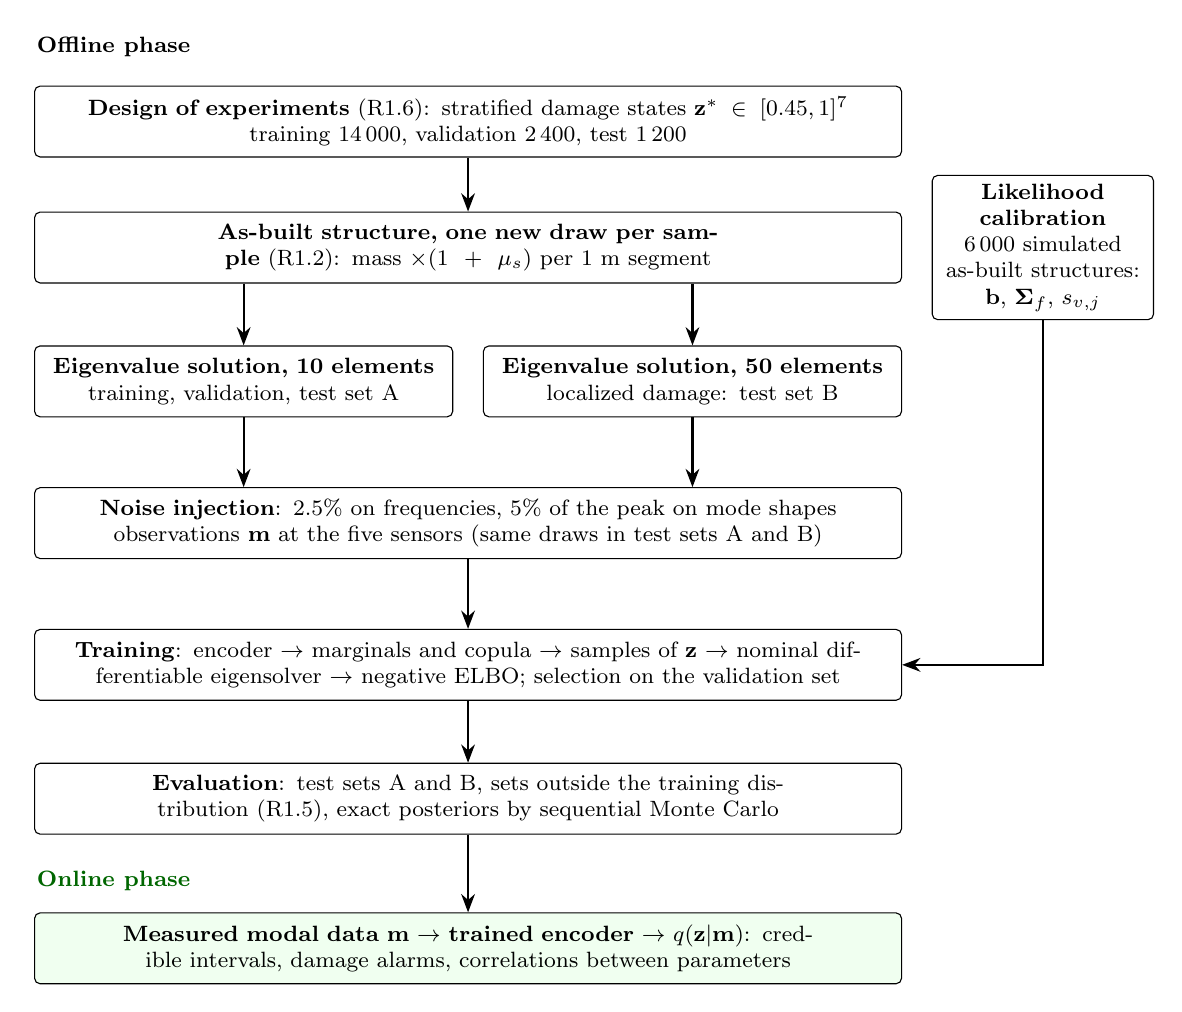
\begin{tikzpicture}[>=Stealth,font=\footnotesize,
  box/.style={draw,rounded corners=2pt,align=center,minimum height=0.9cm,fill=white,inner sep=3pt},
  arr/.style={->,thick}]
  \node[anchor=west,font=\bfseries\footnotesize] at (-5.6,0.95) {Offline phase};
  \node[box,text width=10.8cm] (doe) at (0,0) {\textbf{Design of experiments} (R1.6): stratified damage states $\z^*\in[0.45,1]^7$\\training 14\,000, validation 2\,400, test 1\,200};
  \node[box,text width=10.8cm] (ab) at (0,-1.6) {\textbf{As-built structure, one new draw per sample} (R1.2): mass $\times(1+\mu_s)$ per 1~m segment};
  \node[box,text width=5.1cm] (fe10) at (-2.85,-3.3) {\textbf{Eigenvalue solution, 10 elements}\\training, validation, test set A};
  \node[box,text width=5.1cm] (fe50) at (2.85,-3.3) {\textbf{Eigenvalue solution, 50 elements}\\localized damage: test set B};
  \node[box,text width=10.8cm] (noise) at (0,-5.1) {\textbf{Noise injection}: 2.5\% on frequencies, 5\% of the peak on mode shapes\\observations $\m$ at the five sensors (same draws in test sets A and B)};
  \node[box,text width=10.8cm] (train) at (0,-6.9) {\textbf{Training}: encoder $\to$ marginals and copula $\to$ samples of $\z$ $\to$ nominal differentiable eigensolver $\to$ negative ELBO; selection on the validation set};
  \node[box,text width=10.8cm] (test) at (0,-8.6) {\textbf{Evaluation}: test sets A and B, sets outside the training distribution (R1.5), exact posteriors by sequential Monte Carlo};
  \node[anchor=west,font=\bfseries\footnotesize,green!40!black] at (-5.6,-9.65) {Online phase};
  \node[box,text width=10.8cm,fill=green!6] (on) at (0,-10.5) {\textbf{Measured modal data} $\m$ $\to$ \textbf{trained encoder} $\to$ $q(\z|\m)$: credible intervals, damage alarms, correlations between parameters};
  \node[box,text width=2.6cm] (cal) at (7.3,-1.6) {\textbf{Likelihood calibration}\\6\,000 simulated as-built structures: $\mathbf{b}$, $\bm{\Sigma}_f$, $s_{v,j}$};
  \draw[arr] (doe)--(ab);
  \draw[arr] (fe10 |- ab.south)--(fe10.north);
  \draw[arr] (fe50 |- ab.south)--(fe50.north);
  \draw[arr] (fe10.south)--(fe10 |- noise.north);
  \draw[arr] (fe50.south)--(fe50 |- noise.north);
  \draw[arr] (noise)--(train);
  \draw[arr] (train)--(test);
  \draw[arr] (cal.south) |- (train.east);
  \draw[arr] (test)--(on);
\end{tikzpicture}
\caption{Generation of the synthetic data, offline training and evaluation, and online inference.}
\label{fig:flowchart}
\end{figure}

\begin{action}
New flowchart (Fig.~\tbd{x}, Fig.~\ref{fig:flowchart}) \lines{xx--yy}.
\end{action}

% -----------------------------------------------------------------------------
\begin{rcomment}{6}
Equation 11 ($\mathcal{L}_{\mathrm{freq}}$): The notation $\mathbf{K}_{\mathrm{G}}$ in the decoder function is slightly
confusing since Eq. 5 defines $\hat{\mathbf{K}}_{\mathrm{G}}(\z)$ as the updated stiffness matrix. Please clarify if
$\mathbf{K}_{\mathrm{G}}$ refers to the baseline assembled matrix to avoid confusion with the damaged global matrix.
\end{rcomment}
\pending

% -----------------------------------------------------------------------------
\begin{rcomment}{7}
Sample size in training ($H=1$): In the ``Architecture design and training specifications'' section, it is stated that
a single sample ($H=1$) is drawn during training. While common in VAEs with large batch sizes, please briefly justify why
$H=1$ is sufficient to approximate the expectations in the ELBO loss.
\end{rcomment}

\begin{response}
In the revised implementation, we draw $H=6$ samples of the approximate posterior per observation. With batches of 256
observations, each gradient step uses 1\,536 samples. The Monte Carlo estimate of the loss is unbiased for any $H$, and
$H$ only affects the variance of the gradients. This variance is further reduced because the entropy is computed
exactly, in closed form (Eq.~\eqref{eq:loss}), so that the samples are only used for the expectation of the negative
log-likelihood. The samples are obtained with the closed-form quantile of the truncated normal distribution at the uniform
variables produced by the Gaussian copula. This expression is differentiable with respect to the encoder outputs, and it
replaces the rejection sampling of the submitted version.
% $H$ only affects the variance of the gradients. This variance is further reduced because the entropy is computed
% exactly, in closed form (Eqs.~\eqref{eq:marginal} and~\eqref{eq:loss}), so that the samples are only used for the
% expectation of the negative log-likelihood. The samples are obtained with the closed-form quantile of
% Eq.~\eqref{eq:marginal} at the uniform variables produced by the Gaussian copula. This expression is differentiable with
% respect to the encoder outputs, and it replaces the rejection sampling of the submitted version.
\end{response}
\authornote{optional: a short check of the sensitivity of the results to $H$.}

\begin{action}
Training specifications updated \lines{xx--yy}.
\end{action}

% -----------------------------------------------------------------------------
\begin{rcomment}{8}
Hardware and computational cost: Please report the hardware specifications and the approximate wall-clock time
required for the 11,000 training epochs to provide a practical sense of the computational cost of differentiating the
eigenvalue solver.
\end{rcomment}
\pending
\authornote{report the hardware and wall-clock time of the final training on the GPU server (NVIDIA Quadro GV100 and L40S GPUs; the eigenproblems are solved on the CPU in double precision), measured on an otherwise idle GPU.}

% =============================================================================
\section{References cited in this letter}
% =============================================================================
{\small
\begin{itemize}[leftmargin=*,label={}]
\item El-Borgi, S., Choura, S., Ventura, C., Baccouch, M., Cherif, F. (2005). Modal identification and model updating of a reinforced concrete bridge. Smart Struct.\ Syst.\ 1(1), 83--101.
\item Erduran, E., Nordli, C., Gonen, S. (2022). Effect of elastomeric bearing stiffness on the dynamic response of railway bridges considering vehicle--bridge interaction. Appl.\ Sci.\ 12(23), 11952.
\item Fayyadh, M.M., Abdul Razak, H. (2012). Condition assessment of elastic bearing supports using vibration data. Constr.\ Build.\ Mater.\ 30, 616--628.
\item Garcia-Sanchez, D., Fernandez-Navamuel, A., Zamora S\'anchez, D., Alvear, D., Pardo, D. (2020). Bearing assessment tool for longitudinal bridge performance. J.\ Civil Struct.\ Health Monit.\ 10(5), 1023--1036.
\item Luo, L., Sun, L., Song, M., Liu, J., Li, Y., Xia, Y. (2025). Joint load-parameter-response identification using a physics-encoded neural network. Mech.\ Syst.\ Signal Process.\ 230, 112597.
\item Moliner, E., Mart\'{\i}nez-Rodrigo, M.D., Museros, P. (2017). Dynamic performance of existing double track railway bridges at resonance with the increase of the operational line speed. Eng.\ Struct.\ 132, 98--109.
\item Zuk, W. Bridge vibrations as influenced by elastomeric bearings. Highway Research Board Bulletin 315. \tbd{confirm year and pages}
\item \tbd{Add with the manuscript: EN~1991-2; Teughels et al.\ (2002); Kucukelbir et al.\ (2017); Morningstar et al.\ (2021); Yao et al.\ (2018); Vehtari et al.\ (2024).}
\end{itemize}
}

\end{document}
